% Propósito: mostrar que una curva isofónica se construye mediante juicios de
% igual sonoridad bajo un procedimiento, no mediante igualdad de niveles.
% Origen: definición de curva de igual sonoridad de la sección
% \ref{sec:u7-isofonicas}. No se emplean datos de ISO 226 ni valores
% experimentales.
% Descripción accesible: tres bloques muestran un tono de referencia de
% 1000 Hz, un tono de prueba de frecuencia f cuyo nivel se ajusta y el juicio de
% igual sonoridad. A la derecha, un punto se incorpora a un plano de frecuencia
% y nivel; repetir el procedimiento para distintas frecuencias forma una curva.
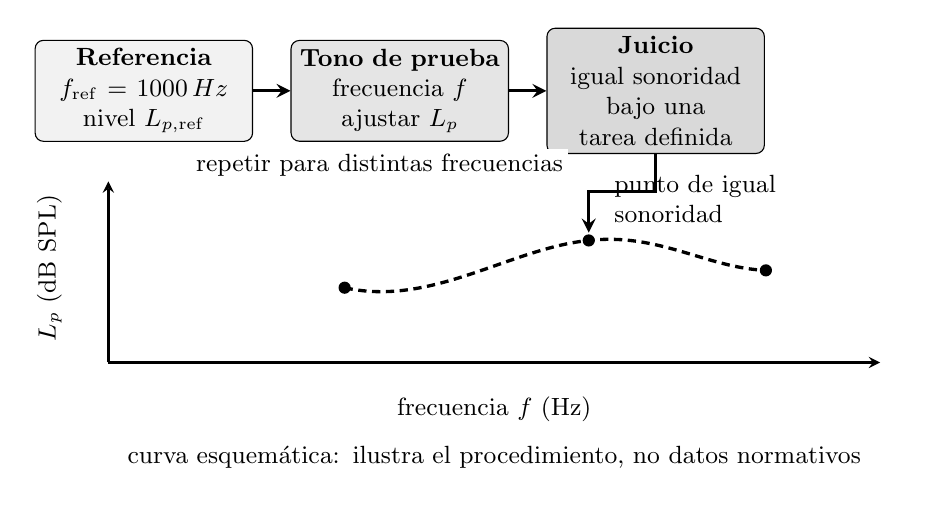
\begin{tikzpicture}[font=\small,>=stealth,x=1cm,y=1cm]
    \tikzset{
        stagebox/.style={draw,rounded corners=3pt,align=center,
            text width=2.55cm,minimum height=1.15cm,inner sep=3pt},
        flow/.style={->,very thick}
    }

    \node[stagebox,fill=black!5] (ref) at (1.55,4.00)
        {\textbf{Referencia}\\
         \(f_\mathrm{ref}=1000\,\text{Hz}\)\\
         nivel \(L_{p,\mathrm{ref}}\)};
    \node[stagebox,fill=black!10] (test) at (4.80,4.00)
        {\textbf{Tono de prueba}\\
         frecuencia \(f\)\\
         ajustar \(L_p\)};
    \node[stagebox,fill=black!15] (judge) at (8.05,4.00)
        {\textbf{Juicio}\\
         igual sonoridad\\
         bajo una tarea definida};

    \draw[flow] (ref.east) -- (test.west);
    \draw[flow] (test.east) -- (judge.west);

    \draw[->,thick] (1.10,0.55) -- (10.90,0.55);
    \draw[->,thick] (1.10,0.55) -- (1.10,2.85);
    \node at (6.00,-0.05) {frecuencia \(f\) (Hz)};
    \node[rotate=90] at (0.35,1.75) {\(L_p\) (dB SPL)};

    \fill (4.10,1.50) circle (2.2pt);
    \fill (7.20,2.10) circle (2.2pt);
    \fill (9.45,1.72) circle (2.2pt);
    \draw[very thick,densely dashed]
        (4.10,1.50) .. controls (5.20,1.25) and (6.20,2.00) ..
        (7.20,2.10) .. controls (8.10,2.20) and (8.70,1.75) ..
        (9.45,1.72);
    \node[anchor=west,align=left,fill=white,inner sep=2pt]
        at (7.45,2.63)
        {punto de igual\\sonoridad};

    \draw[flow] (judge.south) -- ++(0,-0.48) -| (7.20,2.20);
    \node[anchor=east,align=right,fill=white,inner sep=2pt]
        at (6.95,3.05)
        {repetir para distintas frecuencias};
    \node[align=center,text width=10.20cm] at (6.00,-0.65)
        {curva esquemática: ilustra el procedimiento, no datos normativos};
\end{tikzpicture}
